% ============================================================
% 第8章 実証モデルの構築：潜在倒産距離
% ============================================================

\chapter{実証モデルの構築：潜在倒産距離 $Z_{\text{lin}}$ とロジット推定}
\label{chap:empirical_model}

第5章では，潜在倒産距離 $Z_{\text{lin}}$ の構成要素である
収益性 $\mu$，外部ショック感応度 $\sigma$，支援能力 $S$，
倒産閾値 $D$ を実証的に測定可能な変数として定義し，
その採用根拠を整理した。
本章では，これらの変数を用いて $Z_{\text{lin}}$ を
倒産確率モデルに接続するための実証モデルを構築する。

新電力企業の倒産は 0/1 の離散的イベントであり，
Bharath \& Shumway（2008）（以下 B\&S）が示したように，
潜在倒産距離をロジットモデルの latent index として扱うことが
理論的にも実務的にも適切である。
本研究でもこの枠組みを継承し，
$Z_{\text{lin}}$ を倒産確率に写像するロジットモデルを構築する。

以下では，まず本章の目的を整理し（6.1 節），
次に潜在倒産距離 $Z_{\text{lin}}$ を再掲し（6.2 節），
ロジットモデルの定式化（6.3 節），
理論的符号条件（6.4 節），
識別の考え方（6.5 節）を順に示す。

% ---------------------------------------------
% 8.1 本章の目的
% 理論モデル Z_lin を倒産確率モデルに接続するための
% 実証モデル（ロジット）の構築方針を示す節。
% ---------------------------------------------

\section{本章の目的}

第5章では，潜在倒産距離 $Z_{\text{lin}}$ の構成要素である
収益性 $\mu$，外部ショック感応度 $\sigma$，支援能力 $S$，
倒産閾値 $D$ を実証的に測定可能な変数として定義し，
その採用根拠を整理した。
本章では，これらの変数を用いて $Z_{\text{lin}}$ を
倒産確率モデルに接続するための実証モデルを構築する。

新電力企業の倒産は 0/1 の離散的イベントであり，
倒産確率を推定するためには離散選択モデルが必要となる。
Bharath \& Shumway（2008）（以下 B\&S）は，
潜在倒産距離（proxy DD）をロジットモデルの latent index として扱うことで，
Merton 型モデルの構造を維持しつつ，
倒産確率を実務的に推定可能な形に写像した。
本研究もこの枠組みを継承し，
$Z_{\text{lin}}$ をロジットモデルの latent index として扱う。

本章の目的は以下の 3 点である。

\begin{enumerate}
    \item 潜在倒産距離 $Z_{\text{lin}}$ を倒産確率に接続するロジットモデルを定式化すること
    \item $Z_{\text{lin}}$ の構成要素（$\mu, \sigma, S, D$）が倒産確率に与える理論的符号条件を整理すること
    \item モデル推定における識別の考え方を明確化し，第7章の実証分析につなげること
\end{enumerate}

以上により，本章は「理論モデル（第4章）→ 変数定義（第5章）→ 実証推定（第7章）」をつなぐ
中心的な役割を果たす。
次節では，潜在倒産距離 $Z_{\text{lin}}$ を再掲し，
ロジットモデルの latent index としての位置づけを明確にする。

% ---------------------------------------------
% 8.2 潜在倒産距離 Z_lin の再掲
% 第4章で構築した Z_lin を再提示し、
% ロジットモデルの latent index としての位置づけを明確化する節。
% ---------------------------------------------

\section{潜在倒産距離 $Z_{\text{lin}}$ の再掲}

第4章では，Merton モデルおよび Bharath \& Shumway（2008）（以下 B\&S）の
multiplicative → log → linear の構造を基礎として，
新電力企業の倒産構造に適合した潜在倒産距離 $Z_{\text{lin}}$ を理論的に構築した。
また第5章では，その構成要素である収益性 $\mu$，
外部ショック感応度 $\sigma$，支援能力 $S$，倒産閾値 $D$ を
実証的に測定可能な変数として定義した。

本節では，実証モデルの構築に先立ち，
$Z_{\text{lin}}$ の定義を再掲し，
ロジットモデルにおける latent index としての位置づけを明確にする。

\subsection{潜在倒産距離 $Z_{\text{lin}}$ の定義}

本研究が構築する潜在倒産距離は次式で与えられる。



\[
Z_{\text{lin}}
= a\mu - b\sigma + cS - dD + \varepsilon
\]



ここで，

\begin{itemize}
    \item $\mu$：収益性（営業利益率）
    \item $\sigma$：外部ショック感応度（スポット依存度）
    \item $S$：支援能力（親会社・自治体・金融機関による支援の有無）
    \item $D$：倒産閾値（外部ショック時の支払義務）
    \item $\varepsilon$：未観測要因
\end{itemize}

係数の符号条件は理論的に次のように期待される。



\[
a>0,\quad b>0,\quad c>0,\quad d>0
\]



すなわち，収益性と支援能力は倒産距離を押し上げ，
外部ショック感応度と倒産閾値は倒産距離を押し下げる。

\subsection{B\&S の proxy DD との構造的類似性}

B\&S の naive predictor（proxy DD）は，



\[
DD_{\text{naive}}
= \frac{\ln\left(\frac{E+F}{F}\right) + (\hat{\mu}-0.5\hat{\sigma}_V^2)}{\hat{\sigma}_V}
\]



であり，これは



\[
DD \approx a\mu - b\sigma_V + c\ln(V/F)
\]



という線形倒産距離の構造を持つ。

本研究の $Z_{\text{lin}}$ は，この構造を新電力市場に適合する形で再構成したものであり，



\[
\mu \leftrightarrow \text{収益性},\quad
\sigma_V \leftrightarrow \text{外部ショック感応度},\quad
\ln(V/F) \leftrightarrow S - D
\]



という写像関係を持つ。

すなわち，$Z_{\text{lin}}$ は B\&S の proxy DD と同様に，
倒産確率モデルの latent index として機能する。

\subsection{ロジットモデルにおける latent index としての位置づけ}

倒産は 0/1 の離散的イベントであるため，
$Z_{\text{lin}}$ はロジットモデルの latent index として扱われる。

すなわち，



\[
\text{倒産確率} = P(\text{default}=1)
= \Lambda(Z_{\text{lin}})
\]



ここで $\Lambda(\cdot)$ はロジスティック関数である。

このように，$Z_{\text{lin}}$ は
\textbf{理論モデル（第4章）で構築され，変数として定義された（第5章）潜在倒産距離を，
倒産確率に写像するための基礎となる latent index}
として機能する。

次節では，この $Z_{\text{lin}}$ を用いたロジットモデルの定式化を行う。


% ---------------------------------------------
% 8.3 ロジットモデルの定式化
% Z_lin を latent index として倒産確率に写像する
% ロジットモデルの数式と構造を定式化する節。
% ---------------------------------------------

\section{ロジットモデルの定式化}

前節では，潜在倒産距離 $Z_{\text{lin}}$ を再掲し，
その構造が Bharath \& Shumway（2008）（以下 B\&S）の
proxy DD と同様に，倒産確率モデルの latent index として
機能することを確認した。
本節では，この $Z_{\text{lin}}$ を用いて，
倒産確率を推定するロジットモデルを定式化する。

\subsection{倒産確率の基本構造}

新電力企業の倒産は 0/1 の離散的イベントであるため，
倒産確率はロジスティック関数によって次のように表される。



\[
P(\text{default}_i = 1)
= \Lambda(Z_{\text{lin},i})
= \frac{1}{1 + \exp(-Z_{\text{lin},i})}
\]



ここで $\Lambda(\cdot)$ はロジスティック関数であり，
$Z_{\text{lin},i}$ は企業 $i$ の潜在倒産距離である。

\subsection*{latent index としての $Z_{\text{lin}}$}

潜在倒産距離 $Z_{\text{lin}}$ は次式で与えられる。



\[
Z_{\text{lin},i}
= a\mu_i - b\sigma_i + cS_i - dD_i + \varepsilon_i
\]



ここで，

\begin{itemize}
    \item $\mu_i$：収益性
    \item $\sigma_i$：外部ショック感応度
    \item $S_i$：支援能力
    \item $D_i$：倒産閾値
    \item $\varepsilon_i$：未観測要因
\end{itemize}

この構造は，B\&S の proxy DD が latent index として
ロジットモデルに組み込まれた構造と同一である。

すなわち，



\[
\text{default}_i^*
= Z_{\text{lin},i}
\quad\Rightarrow\quad
\text{default}_i
=
\begin{cases}
1 & \text{if } Z_{\text{lin},i} > 0 \\
0 & \text{otherwise}
\end{cases}
\]



という latent variable モデルの枠組みを採用する。

\subsection{推定式の明示}

以上をまとめると，本研究が推定するロジットモデルは次式で表される。



\[
P(\text{default}_i = 1)
= \frac{1}{1 + \exp\left[-(a\mu_i - b\sigma_i + cS_i - dD_i)\right]}
\]



あるいは logit 形式で書くと，



\[
\log\left(\frac{P(\text{default}_i = 1)}{1 - P(\text{default}_i = 1)}\right)
= a\mu_i - b\sigma_i + cS_i - dD_i
\]



となる。

この式は，Merton 型モデルの multiplicative → log → linear の構造を
B\&S の proxy 化の思想に基づき離散時間に写像したものであり，
新電力企業の倒産構造に適合する形で再構成された倒産確率モデルである。



% ---------------------------------------------
% 8.4 相互作用項を導入した拡張ロジットモデル
% ・μ×σ、S×D の相互作用をロジット式に組み込む
% ・第7章の相互関係シミュレーションと整合
% ・第9章のロバストネス分析への橋渡し
% ---------------------------------------------

\section{相互作用項を導入した拡張ロジットモデル}

前節では，潜在倒産距離 $Z_{\text{lin}}$ を latent index とする
基本ロジットモデルを定式化した。
しかし，倒産リスクは単一要因の線形効果だけで決まるわけではなく，
複数の要因が同時に変化することで非線形的に増幅・緩和される場合が多い。
第6章の相互関係シミュレーションでも示したように，
特に以下の 2 つの相互作用が倒産確率に強く影響する。

\begin{itemize}
    \item 収益性 $\mu$ と外部ショック感応度 $\sigma$ の相互作用（$\mu \cdot \sigma$）
    \item 支援能力 $S$ と倒産閾値 $D$ の相互作用（$S \cdot D$）
\end{itemize}

これらをロジットモデルに組み込むと，拡張版の latent index は次式で表される。



\[
Z_{\text{int},i}
= a\mu_i - b\sigma_i + cS_i - dD_i
+ \gamma_{\mu\sigma}(\mu_i \cdot \sigma_i)
+ \gamma_{SD}(S_i \cdot D_i)
\]



ここで，
\begin{itemize}
    \item $\gamma_{\mu\sigma}$：収益性が市場ショックの悪影響をどの程度緩和するか
    \item $\gamma_{SD}$：支援能力が負債過多の悪影響をどの程度吸収するか
\end{itemize}
を表す。

倒産確率は次式で与えられる。



\[
P(\text{default}_i = 1)
= \Lambda(Z_{\text{int},i})
\]



この拡張モデルは，第6章で示した相互関係シミュレーションの結果と整合的であり，
特に以下の含意を持つ。

\begin{itemize}
    \item $\gamma_{\mu\sigma} < 0$ が推定されれば，
          「収益性が高い企業ほど市場ショックに強い」ことを意味する。
    \item $\gamma_{SD} > 0$ が推定されれば，
          「支援能力が高い企業ほど負債過多の悪影響を吸収できる」ことを意味する。
\end{itemize}

% ------------------------------------------------------------
% 相互作用項の可視化（μ×σ）
% ------------------------------------------------------------

\begin{figure}[H]
    \centering
    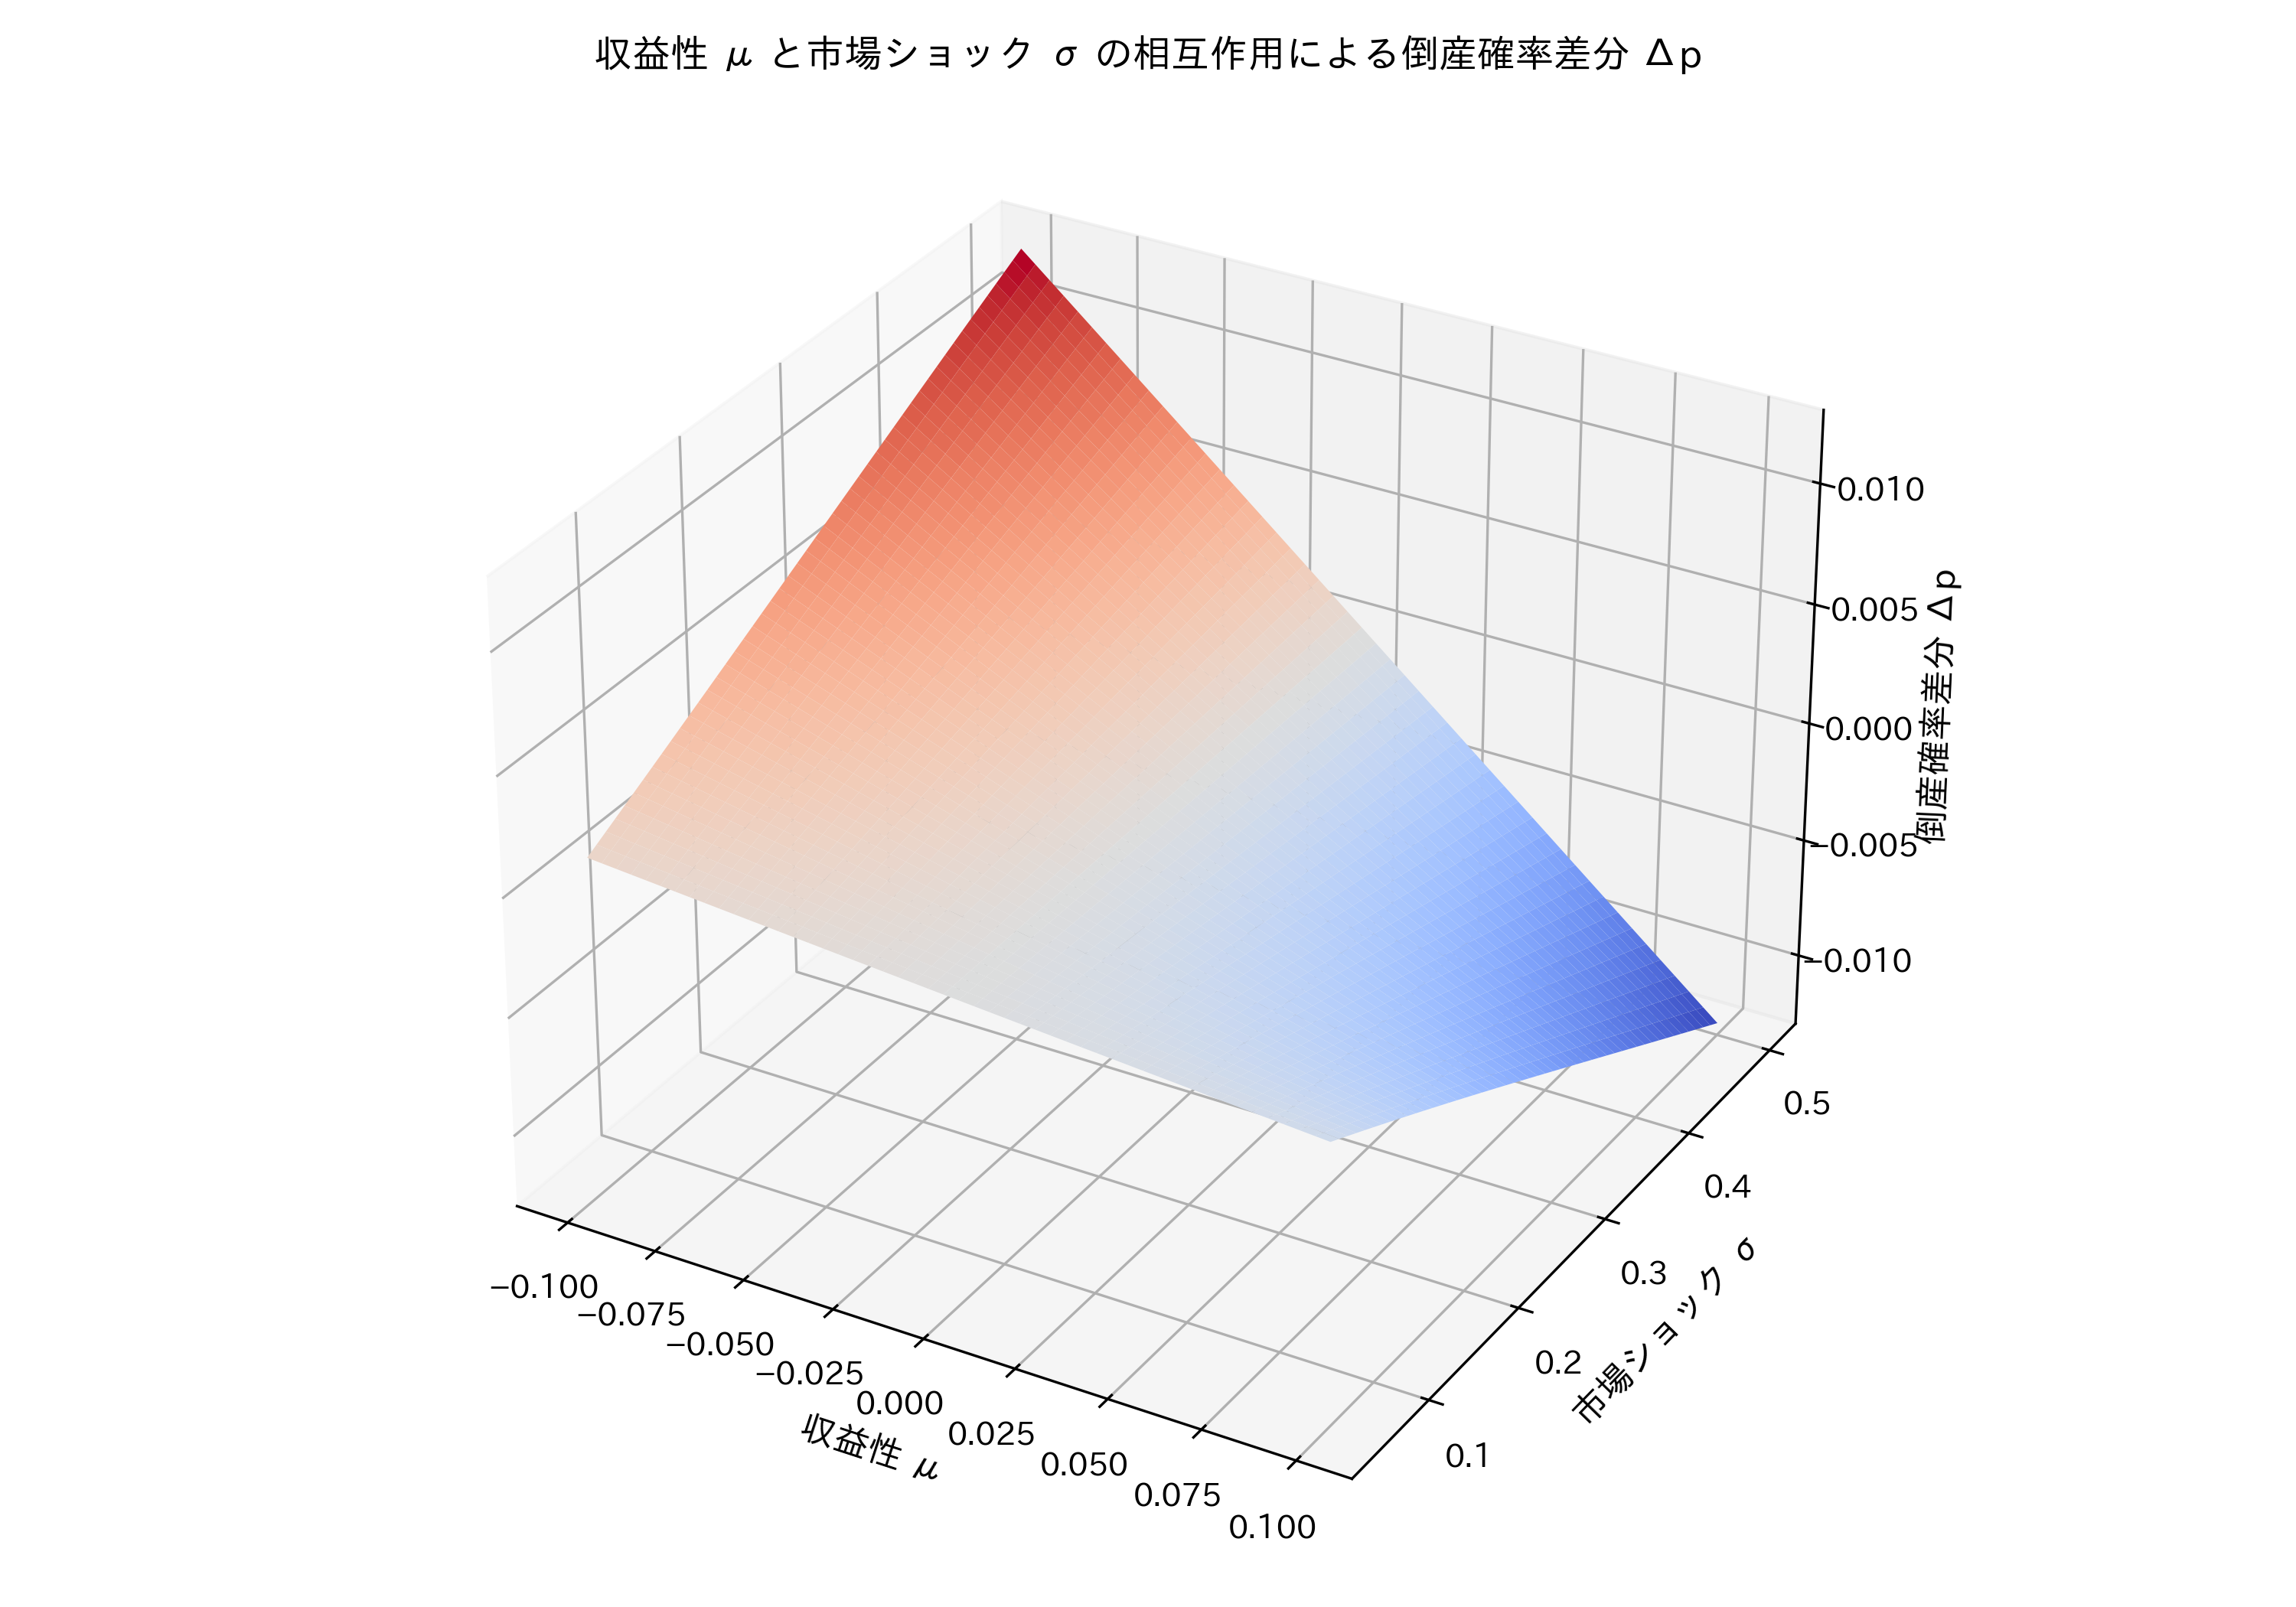
\includegraphics[width=0.80\linewidth]{figures/interaction_mu_sigma_surface.png}
    \caption{収益性 $\mu$ と市場ショック $\sigma$ の相互作用による倒産確率差分 $\Delta p$ の3Dサーフェス}
    \label{fig:interaction_mu_sigma_surface_ch7}
\end{figure}

図\ref{fig:interaction_mu_sigma_surface_ch7} は，
収益性 $\mu$ と外部ショック感応度 $\sigma$ の相互作用項
$\gamma_{\mu\sigma}(\mu \cdot \sigma)$ が倒産確率に与える影響を可視化したものである。
$\mu$ が低く $\sigma$ が高い領域で $\Delta p$ が大きくなることから，
収益性が低い企業ほど市場ショックの悪影響が増幅されることが確認できる。
一方，$\mu$ が高い領域では $\sigma$ の影響が緩和され，
相互作用項が倒産確率を大きく押し下げる。
これは $\gamma_{\mu\sigma}<0$ という符号条件と整合的である。

% ------------------------------------------------------------
% 相互作用項の可視化（S×D）
% ------------------------------------------------------------

\begin{figure}[H]
    \centering
    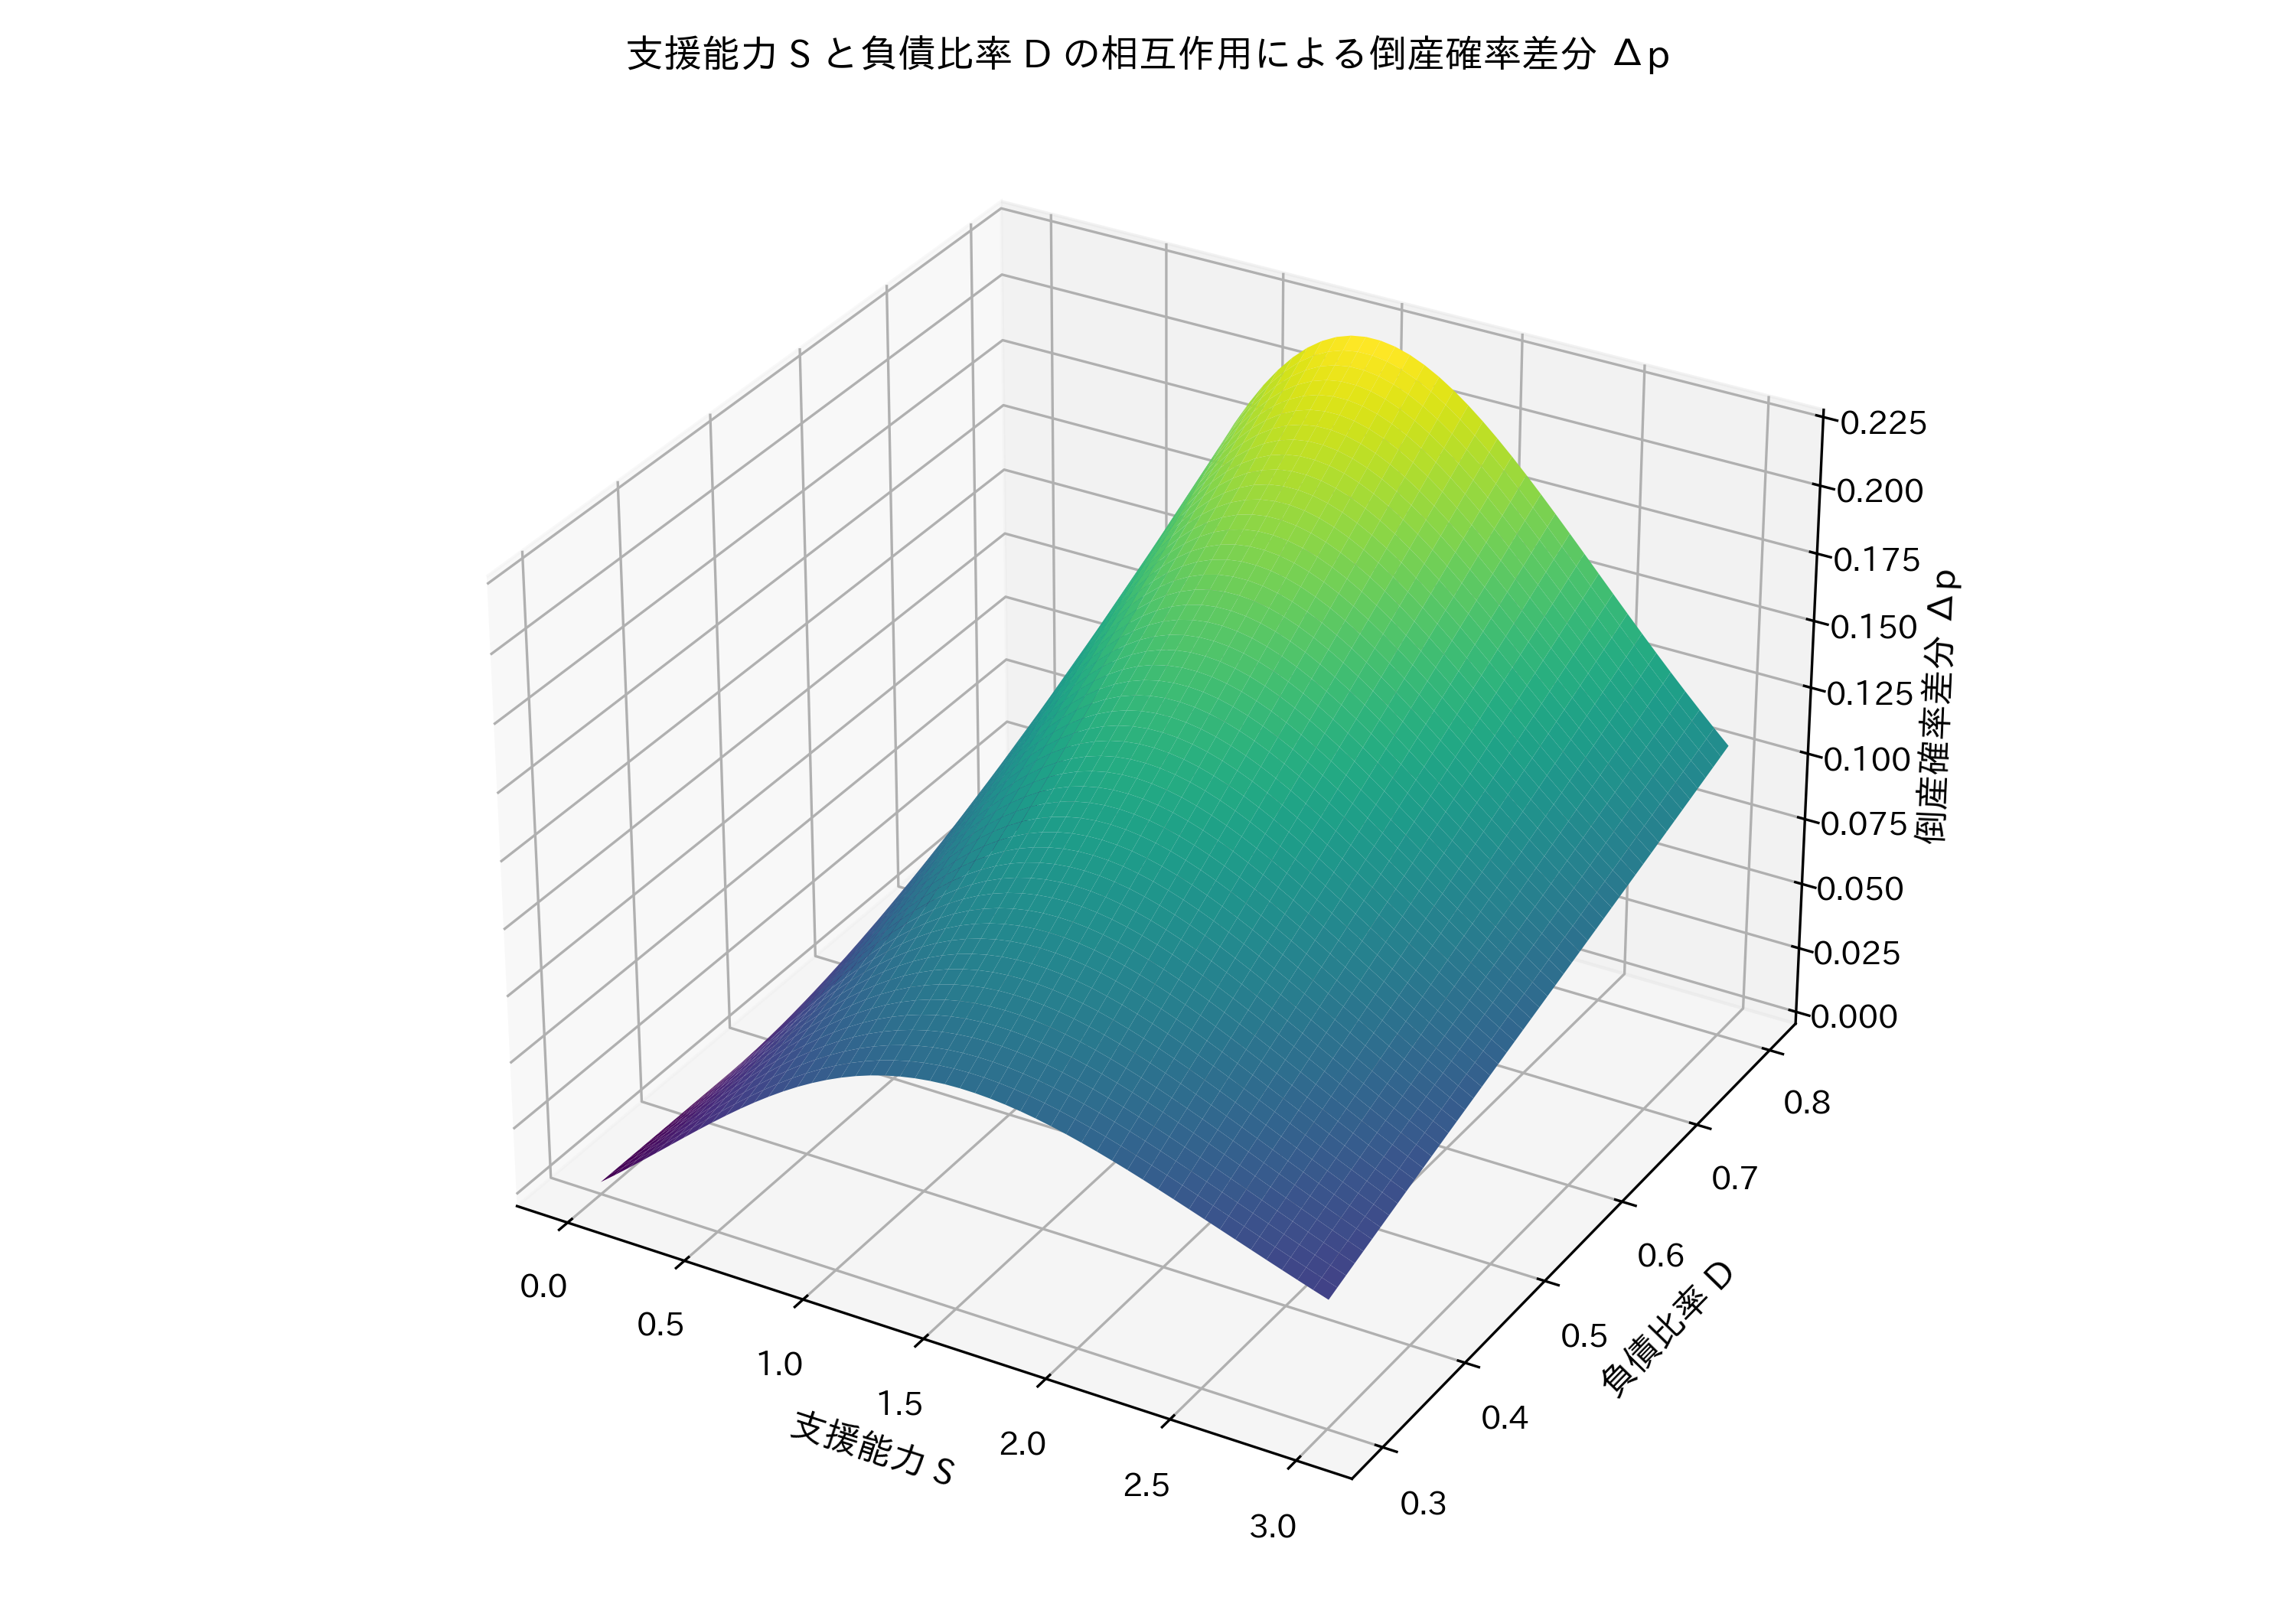
\includegraphics[width=0.80\linewidth]{figures/interaction_S_D_surface.png}
    \caption{支援能力 $S$ と負債比率 $D$ の相互作用による倒産確率差分 $\Delta p$ の3Dサーフェス}
    \label{fig:interaction_S_D_surface_ch7}
\end{figure}

図\ref{fig:interaction_S_D_surface_ch7} は，
支援能力 $S$ と倒産閾値 $D$ の相互作用項
$\gamma_{SD}(S \cdot D)$ が倒産確率に与える影響を可視化したものである。
$S$ が高い企業では，$D$ の上昇による倒産確率の悪化が大幅に緩和され，
$\Delta p$ が正の plateau（高原）として現れる。
一方，$S=0$ の企業では $D$ の悪影響がそのまま倒産確率に反映され，
$\Delta p$ はほぼゼロとなる。
これは $\gamma_{SD}>0$ という符号条件と整合的である。

以上の可視化は，相互作用項をロジットモデルに導入する理論的根拠を補強し，
次節で整理する符号条件および第8章のロバストネス分析への橋渡しとなる。


\subsection*{ロジットモデルを採用する理由}

ロジットモデルを採用する理由は以下の通りである。

\begin{itemize}
    \item 倒産は 0/1 の離散的イベントであり，ロジットは標準的手法である
    \item B\&S が proxy DD をロジットで推定しており，理論的整合性が高い
    \item $Z_{\text{lin}}$ の線形構造が logit の latent index として自然に解釈できる
    \item 係数の符号条件（$a>0, b>0, c>0, d>0$）が明確で，仮説検証に適している
\end{itemize}

以上により，ロジットモデルは，
本研究の潜在倒産距離 $Z_{\text{lin}}$ を倒産確率に接続するための
最も自然かつ理論的に整合的な推定手法である。

次節では，$Z_{\text{lin}}$ の構成要素が倒産確率に与える
理論的符号条件を整理する。



% ---------------------------------------------
% 8.5 符号条件（理論的期待値）
% Z_lin の各構成要素（μ, σ, S, D）が倒産確率に
% どのような符号で影響するかを理論的に整理する節。
% ---------------------------------------------

\section{理論的符号条件}

本節では，本研究で構築した倒産リスクモデルにおける主要変数
（収益性 $\mu$，外部ショック感応度 $\sigma$，支援能力 $S$，倒産閾値 $D$）
が，倒産確率に対してどのような符号を持つべきかを理論的に整理する。

ここで重要なのは，単に「収益性が高ければ倒産しにくい」といった
自明な経験則を述べることではない。
むしろ，本研究が明らかにしたいのは，
新電力企業に特有の市場構造・制度構造が，
これらの変数を通じて倒産確率にどのような
\textbf{構造的な作用}を及ぼすのかという点である。

\subsection*{収益性 $\mu$ の符号：倒産確率を低下させる（$-$）}

収益性 $\mu$ は，企業価値のドリフト項として，
将来キャッシュフローの期待成長率を表す。
Merton 型の構造モデルにおいては，
企業価値の期待成長率が高いほど，
負債返済に必要な閾値を上回る確率が高まるため，
倒産確率は低下する。

新電力企業の場合，$\mu$ は単なる営業利益率ではなく，
\textbf{調達戦略・顧客構成・契約単価の持続可能性を含む「事業の質」}を反映する。
したがって $\mu$ の符号は，
新電力市場の構造的脆弱性を緩和する方向に作用するという
経済的意味を持つ。

\subsection*{外部ショック感応度 $\sigma$ の符号：倒産確率を上昇させる（$+$）}

$\sigma$ は，市場価格や制度コストの変動が
企業キャッシュフローにどれほど波及するかを表す。
Merton モデルでは，ボラティリティが高いほど
企業価値が閾値を下回る確率が増えるため，
倒産確率は上昇する。

新電力企業では，$\sigma$ は
\textbf{スポット市場依存度，需給調整金の影響度，短期契約比率}
といった制度的要因によって決定される。
これは他産業には見られない特徴であり，
単なる「リスクが高いほど倒産しやすい」という一般論ではなく，
\textbf{制度設計そのものが倒産確率の符号を規定している}点に
本研究の理論的意義がある。

\subsection*{支援能力 $S$ の符号：倒産確率を低下させる（$-$）}

$S$ は，親会社・自治体・金融機関などの
外生的支援主体の存在を表す。
これは従来の倒産研究では明示的に扱われてこなかった要因である。

新電力企業は，外部ショックが即時に資金繰りへ波及するため，
\textbf{内部留保では吸収できないショックを外部資本で緩和できるかどうか}
が生死を分ける。
したがって $S$ の符号は，
単なる財務指標では捉えられない
\textbf{制度的・組織的な耐性}を反映している。

\subsection*{倒産閾値 $D$ の符号：倒産確率を上昇させる（$+$）}

$D$ は，外部ショック時に必要となるキャッシュアウトや
制度コストの増加によって決まる倒産ラインである。
制度変更や需給逼迫によって $D$ が上昇すると，
企業価値が閾値を下回る確率が高まり，
倒産確率は上昇する。

ここで重要なのは，
\textbf{新電力市場では $D$ が外生的に変動する}という点である。
これは従来の倒産モデルが前提としてきた
「固定的な倒産閾値」とは根本的に異なる。
本研究の理論モデルは，
この制度的特徴を明示的に取り込むことで，
新電力企業の倒産急増を説明する枠組みを提供する。

\subsection*{まとめ}

以上より，本研究の符号条件は単なる経験則ではなく，
新電力市場に特有の制度構造・市場構造を踏まえた
\textbf{構造的な倒産メカニズム}を反映している。
すなわち，$\mu$・$\sigma$・$S$・$D$ の符号は，
倒産確率の方向性を示すだけでなく，
新電力企業の倒産が従来モデルでは説明できない理由を
理論的に裏付ける役割を果たす。


% ---------------------------------------------
% 8.6 識別の考え方（Ordered Logit と整合した完全版）
% ---------------------------------------------

\section{識別の考え方}

本節では，Ordered Logit モデルを推定する際に，
潜在倒産距離 $Z_{\text{lin}}$ の構成要素
（収益性 $\mu$，外部ショック感応度 $\sigma$，支援能力 $S$，倒産閾値 $D$）
がどのように識別されるかを整理する。
識別の明確化は，推定結果の解釈可能性を担保するうえで不可欠であり，
本研究の構造モデル（第4章），潜在変数モデル（第5章），
および潜在倒産距離の挙動を可視化した第7章のシミュレーションと
整合的な推定戦略を構築するための基盤となる。

\subsection{Ordered Logit における識別：latent index と cutpoints}

本研究では倒産ステージを


\[
y \in \{0,1,2,3\}
\]


という順序尺度として扱うため，
連続的倒産距離 $Z_{\text{lin}}$ は Ordered Logit の latent index として
次式の潜在変数モデルに組み込まれる。



\[
y^*_i = Z_{\text{lin},i}
\]



観測される倒産ステージは，cutpoints（閾値）


\[
\tau_1 < \tau_2 < \tau_3
\]


によって次のように決定される。



\[
y_i =
\begin{cases}
0 & \text{if } y^*_i \le \tau_1 \\
1 & \text{if } \tau_1 < y^*_i \le \tau_2 \\
2 & \text{if } \tau_2 < y^*_i \le \tau_3 \\
3 & \text{if } y^*_i > \tau_3
\end{cases}
\]



したがって，識別は
\begin{itemize}
    \item latent index（$Z_{\text{lin}}$ の係数）
    \item cutpoints（$\tau_1,\tau_2,\tau_3$）
\end{itemize}
の二種類のパラメータが独立に推定されることで保証される。

第7章で可視化した $Z_{\text{lin}}$ の地形は，
この latent index $y^*$ の挙動そのものであり，
Ordered Logit の識別構造と直接対応している。

\subsection{制度構造に基づく識別：四要素の独立性}

$Z_{\text{lin}}$ の構成要素は，新電力市場の制度構造において
明確に異なる経路で倒産に影響するため，
識別可能性が高い。

\begin{itemize}
    \item $\mu$（収益性）：企業内部の収益構造・事業の質を反映
    \item $\sigma$（外部ショック感応度）：スポット依存度や調達戦略といった市場構造を反映
    \item $S$（支援能力）：親会社・自治体・金融機関による外生的支援主体の存在
    \item $D$（倒産閾値）：インバランス負担や制度コストといった外生的支払義務
\end{itemize}

これらは制度的にも経済的にも異なる要因であり，



\[
\mu \not\leftrightarrow \sigma,\qquad
S \not\leftrightarrow D
\]



という構造的独立性が識別を支えている。

第2章で観察した倒産企業（F-Power，ウエスト電力など）においても，
これら四要素は明確に異なる経路で財務悪化を引き起こしており，
実際の倒産構造が識別可能性を裏付けている。

\subsection{多重共線性の回避：概念的区別と制度的区別}

多重共線性の可能性として最も注意すべきは，
外部ショック感応度 $\sigma$ と倒産閾値 $D$ の関係である。



\[
\sigma = \text{スポット依存度},\qquad
D = \text{インバランス負担 + 調達費用急騰幅}
\]



両者は概念的に異なるだけでなく，
制度的にも異なる要因によって決定されるため，
識別性は制度的に確保される。

第2章の観察でも，
F-Power は $\sigma$ が高く，ウエスト電力は $D$ が高いなど，
企業ごとに異なる構造的弱点が確認されており，
これが識別の実証的根拠となる。

\subsection{外生性の確保：制度的・組織的要因の利用}

Ordered Logit 推定における外生性の確保は重要である。

\begin{itemize}
    \item $\mu$（収益性）は倒産前の財務データに基づくため外生的
    \item $\sigma$（外部ショック感応度）は調達構造に基づき，倒産と同時決定されない
    \item $S$（支援能力）は親会社・自治体の判断に依存し，企業内部要因と独立
    \item $D$（倒産閾値）は制度的支払義務であり，企業行動と独立
\end{itemize}

特に $S$ と $D$ は制度的・外生的要因であり，
倒産ステージとの同時決定性の懸念が小さい。

\subsection{クロスセクションによる識別}

本研究のデータ構造は以下の特徴を持つ。

\begin{itemize}
    \item 倒産は 1 回限りのイベントであり，企業ごとの時系列は短い
    \item 外部ショック（JEPX 価格急騰）は特定期間に集中して発生
    \item 企業間の調達構造・支援能力には大きなクロスセクション差がある
\end{itemize}

したがって，識別の中心はクロスセクション差に依存する。

特に，



\[
\sigma_i,\ S_i,\ D_i
\]



の企業間差が大きいため，
Ordered Logit 推定における識別は十分に確保される。

\subsection{B\&S の識別戦略との比較：制度構造の拡張}

B\&S の識別戦略は，

\begin{itemize}
    \item $\mu$：過去リターン
    \item $\sigma_V$：株価ボラティリティ
    \item $F$：帳簿価値負債
\end{itemize}

という異なる情報源に基づいており，
本研究の識別戦略と構造的に類似している。

しかし，新電力企業は株価データを持たず，
制度コストが外生的に変動するため，
本研究では，

\begin{itemize}
    \item $\mu$：財務データ
    \item $\sigma$：調達構造データ
    \item $S$：政策・親会社情報
    \item $D$：制度的支払義務データ
\end{itemize}

という制度構造に基づく識別戦略を採用する。
これは B\&S の単なる模倣ではなく，
制度構造を明示的に取り込んだ拡張である。

\subsection{識別のまとめ}

以上より，本研究の Ordered Logit モデルは以下の点で識別可能である。

\begin{itemize}
    \item latent index（$Z_{\text{lin}}$）と cutpoints（$\tau_1,\tau_2,\tau_3$）が独立に推定される
    \item 四要素（$\mu, \sigma, S, D$）が制度的・経済的に独立している
    \item 多重共線性の懸念が制度的区別により小さい
    \item 外生性が制度的に確保されている
    \item クロスセクション差が大きく，識別に十分な変動がある
    \item 第2章の倒産事例観察が，識別の実証的根拠を提供している
\end{itemize}

以上により，本研究の Ordered Logit モデルは
理論的にも実証的にも識別可能であり，
第9章の実証分析に適用可能である。
